%----------------------------------------------------------------------------
\chapter{Data processing}\label{sect:DataProcessing}
%----------------------------------------------------------------------------
\section{CNN and Daily Mail data}
%----------------------------------------------------------------------------
The most widely used dataset on the field of summarization is the \textit{CNN - Daily Mail} dataset.
This dataset contains over 300,000 articles and their respective summaries from Daily Mail articles collected from June 2010 to April 2015 and CNN news collected from April 2007 until the end of April 2015.~\cite{CNN_DM}

The only downside is that the summaries are not strictly extracted from the article hence there are expressions in the summaries that may not appear in the original article.

There are multiple preprocessed versions available on this dataset. The dataset I used consists of the articles, their corresponding highlights and also the set of sentences from each article, that together give the highest achievable ROUGE score using the naive greedy method described in the following subsection. I will reference these summaries as the extracted summary of an article.

\subsection{Greedy algorithm}
The (naive) greedy method works with a very basic main principle, always choose the sentence, that maximizes the ROUGE score of the summary.

It's important to note, that it is not a summarization method, it only gives us the highest achievable ROUGE score on a given dataset.

\begin{algorithm}
	\SetAlgoLined
	\KwResult{The n best sentence from the text}
	best\_sentences = ""\;
	\While{i < number of required sentences}{
		rouge\_scores = map()\;
		\ForEach{sentence in text \(\notin\) best\_sentences}{
			rouge\_scores[concat(best\_sentences, sentence)] =  rouge\_score(sentence)\;
		}
		best\_sentence = max\_key\_by\_value(rouge\_scores)\;
		best\_sentences = concat(best\_sentences, best\_sentence)\;
		i = i + 1\;
	}
	\caption{Greedy summarization algorithm}
\end{algorithm}

\begin{table}[!ht]
	\centering
	\begin{tabular}{| l | l |}
		\hline
		\textbf{Evaluation method}&\textbf{Score}\\ \hline \hline
		\textbf{ROUGE-1}&73.91\\ \hline
		\textbf{ROUGE-2}&39.29 \\ \hline
		\textbf{ROUGE-L}&51.01 \\ \hline
		\textbf{ROUGE-SU*}&49.35 \\ \hline
	\end{tabular}
	\caption{ROUGE scores of the top 4 sentences chosen by the naive greedy algorithm over the test set of the CNN-Daily Mail data}
	\label{tab:extr}
\end{table}
As the table~\ref{tab:extr} shows this method works surprisingly well. There have been some advancement of this method regarding its speed~\cite{GreedySum}.

\subsection{Gensim Benchmark}
As I mentioned before, I used the output of gensim's TextRank based summarization method as my benchmark for the graph neural network model evaluation.
\begin{table}[!ht]
	\centering
	\begin{tabular}{| l | l |}
		\hline
		\textbf{Evaluation method}&\textbf{Score}\\ \hline \hline
		\textbf{ROUGE-1}&56.35 \\ \hline
		\textbf{ROUGE-2}&20.80 \\ \hline
		\textbf{ROUGE-L}&34.47 \\ \hline
		\textbf{ROUGE-SU*}&29.27 \\ \hline
	\end{tabular}
	\caption{ROUGE scores of the top 4 sentences chosen by the gensim library's TextRank variation based summarization algorithm over the test set of the CNN-Daily Mail data}
\end{table}
\FloatBarrier

\subsection{Example from the dataset}\label{subsect:example}
\textbox{\textbf{Article}

Usain Bolt rounded off the world championships Sunday by claiming his third gold in Moscow as he anchored Jamaica to victory in the men's 4x100m relay. The fastest man in the world charged clear of United States rival Justin Gatlin as the Jamaican quartet of Nesta Carter, Kemar Bailey-Cole, Nickel Ashmeade and Bolt won in 37.36 seconds. The U.S finished second in 37.56 seconds with Canada taking the bronze after Britain were disqualified for a faulty handover. The 26-year-old Bolt has now collected eight gold medals at world championships, equaling the record held by American trio Carl Lewis, Michael Johnson and Allyson Felix, not to mention the small matter of six Olympic titles. The relay triumph followed individual successes in the 100 and 200 meters in the Russian capital. "I'm proud of myself and I'll continue to work to dominate for as long as possible," Bolt said, having previously expressed his intention to carry on until the 2016 Rio Olympics. Victory was never seriously in doubt once he got the baton safely in hand from Ashmeade, while Gatlin and the United States third leg runner Rakieem Salaam had problems. Gatlin strayed out of his lane as he struggled to get full control of their baton and was never able to get on terms with Bolt. Earlier, Jamaica's women underlined their dominance in the sprint events by winning the 4x100m relay gold, anchored by Shelly-Ann Fraser-Pryce, who like Bolt was completing a triple. Their quartet recorded a championship record of 41.29 seconds, well clear of France, who crossed the line in second place in 42.73 seconds. Defending champions, the United States, were initially back in the bronze medal position after losing time on the second handover between Alexandria Anderson and English Gardner, but promoted to silver when France were subsequently disqualified for an illegal handover. The British quartet, who were initially fourth, were promoted to the bronze which eluded their men's team. Fraser-Pryce, like Bolt aged 26, became the first woman to achieve three golds in the 100-200 and the relay. In other final action on the last day of the championships, France's Teddy Tamgho became the third man to leap over 18m in the triple jump, exceeding the mark by four centimeters to take gold. Germany's Christina Obergfoll finally took gold at global level in the women's javelin after five previous silvers, while Kenya's Asbel Kiprop easily won a tactical men's 1500m final. Kiprop's compatriot Eunice Jepkoech Sum was a surprise winner of the women's 800m. Bolt's final dash for golden glory brought the eight-day championship to a rousing finale, but while the hosts topped the medal table from the United States there was criticism of the poor attendances in the Luzhniki Stadium. There was further concern when their pole vault gold medalist Yelena Isinbayeva made controversial remarks in support of Russia's new laws, which make "the propagandizing of non-traditional sexual relations among minors" a criminal offense. She later attempted to clarify her comments, but there were renewed calls by gay rights groups for a boycott of the 2014 Winter Games in Sochi, the next major sports event in Russia.

\textbf{Summary}

Usain Bolt wins third gold of world championship

Anchors Jamaica to 4x100m relay victory

Eighth gold at the championships for Bolt

Jamaica double up in women's 4x100m relay

\textbf{Extracted summary}

Usain Bolt rounded off the world championships Sunday by claiming his third gold in Moscow as he anchored Jamaica to victory in the men's 4x100m relay.

The fastest man in the world charged clear of United States rival Justin Gatlin as the Jamaican quartet of Nesta Carter, Kemar Bailey-Cole, Nickel Ashmeade and Bolt won in 37.36 seconds.

Earlier, Jamaica's women underlined their dominance in the sprint events by winning the 4x100m relay gold, anchored by Shelly-Ann Fraser-Pryce, who like Bolt was completing a triple.

Their quartet recorded a championship record of 41.29 seconds, well clear of France, who crossed the line in second place in 42.73 seconds.
}

As you can see the extracted summary contains the four best sentences from the article.
%----------------------------------------------------------------------------
\section{Universal Dependencies}
%----------------------------------------------------------------------------
Before we discuss the data processing steps any further I need to clarify what Universal Dependencies are, and why are they useful.

\begin{figure}[!ht]
	\centering
	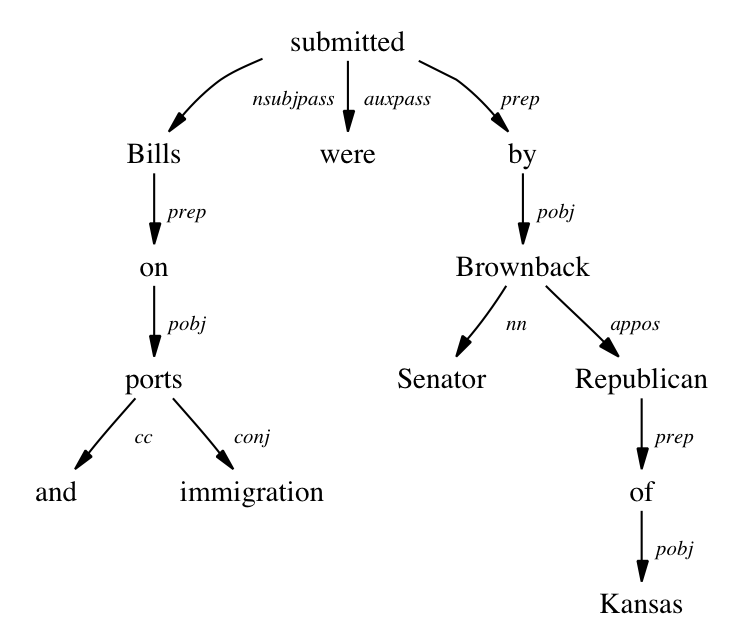
\includegraphics[width=100mm, keepaspectratio]{figures/UD.png}
	\caption{UD graph of "\textit{Bills on ports and immigration were submitted by Senator Brownback, Republican of Kansas.}" Image from \href{https://nlp.stanford.edu/software/stanford-dependencies.shtml}{the Stanford site}}
	\label{fig:UD}
\end{figure}

Universal dependency trees represent the grammatical relationships between the words of a sentence; it gives us the grammatical dependencies between words. They can be easily interpreted with some knowledge of the grammatical structure of languages and they are widely used because of this. UD graphs are highly standardized and are a language independent way to generate the grammatical structure.

One example of a dependency parsed sentence is on Figure~\ref{fig:UD}\footnote{https://nlp.stanford.edu/software/stanford-dependencies.shtml}. You can see the connections and their types between words. Some dependency parsers also predict part-of-speech (POS) tags. For this example sentence the POS tags are the following:
\textbox{Bills: \textit{noun}, on: \textit{preposition}, ports: \textit{noun}, and: \textit{conjunction}, immigration: \textit{noun}, were: \textit{verb}, submitted: \textit{verb}, by: \textit{preposition}, Senator: \textit{noun}, Brownback: \textit{noun}, Republican: \textit{noun}, of: \textit{preposition}, Kansas: \textit{noun}}{}

Dependency trees have been used from the early 20th century based on the work of Lucien Tesni\`ere. In his book titled \textit{\'El\'ements de syntaxe structurale} (Elements of Structural Syntax)\cite{UD} he described the modern grammatical dependency graph structure.

We construct these trees by dependency parsing. There is a multitude of ways we can do that, the library I used in my solution (\href{https://github.com/stanfordnlp/stanfordnlp}{stanfordnlp})\footnote{https://github.com/stanfordnlp/stanfordnlp} utilizes the deep learning based approach.

Most UD parsing methods use treebanks built from parsed corpora, and are used for annotation. Treebanks have been standardized in 2013 by Ryan McDonald's team~\cite{TextRank}. Treebanks are available in multiple languages on the \href{https://universaldependencies.org/}{universal dependency site}.\footnote{\url{https://universaldependencies.org/}} There was a shared task~\cite{ParserSharedTask} to build a parser that is capable of dependency parsing in multiple languages.

%----------------------------------------------------------------------------
\section{Graph format}
%----------------------------------------------------------------------------

The graph\_nets library was developed and published on \href{https://github.com/deepmind/graph_nets}{GitHub}\footnote{\url{https://github.com/deepmind/graph_nets}} by DeepMind in 2018. The team detailed their solutions in the publication titled \textit{Relational inductive biases, deep learning, and graph networks}~\cite{GraphNet}. The graph network was defined to learn graph transformations between relational data. Such relational data can be data from physical systems, sorting problems, shortest path problems.\footnote{\url{https://github.com/deepmind/graph_nets/tree/master/graph_nets/demos}} At first it was not clear whether they can be efficiently trained on real-world data,\footnote{\url{https://github.com/deepmind/graph\_nets/issues/36}} but experiments quickly showed, it can be trained with appropriate relational data.

I defined the extractive summarization as graph transformation, where the input graph is the merged article graph and the output is the said article graph with the nodes and edges that are in the summary graph marked with one and the ones not in the summary graph marked with zero. I used the graph\_nets library to train graph neural networks to learn this graph transformation.
	
The graph\_nets library uses a specific format for graphs, a so called GraphTuple. The user can transform multiple graphs with networkx format or dictionary	 to a GraphTuple object. In my project I used dictionaries because they seemed to be the more straightforward and manageable approach.
The graph dictionary contains the following elements:
\begin{itemize}
	\item nodes: list containing the feature vectors of each node. In my final solution each node's feature vector is the lemma and the part-of-speech tag of the given word 
	\item edges: list containing the feature vectors of each edge. The final feature vector contains the type of each word relation.
	\item globals: global parameter list. I found no relevant use for this parameter in my project.
	\item senders: list containing the indices of the sender nodes in the order of the edges.
	\item receivers: list containing the indices of the receiver nodes in the order of the edges.
\end{itemize}

\begin{figure}[!ht]
	\centering
	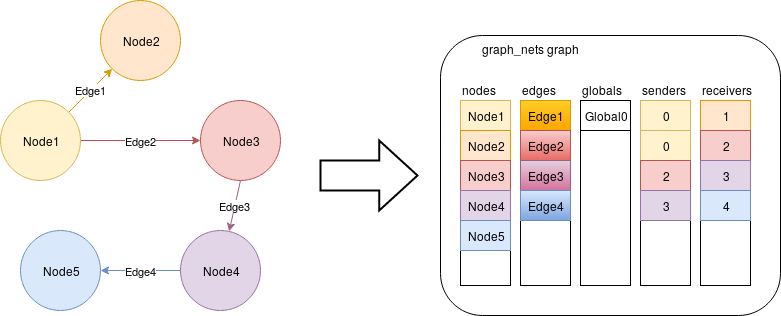
\includegraphics[width=150mm, keepaspectratio]{figures/transform_color.png}
	\caption{Graph transformation to dictionary format.}
	\label{fig:transform_graph}
\end{figure}

On the visual representation Figure \ref{fig:transform_graph} of this kind of graph transformation I highlighted the nodes and edges and the corresponding feature vectors and indices with the same color for easy traceability.
\FloatBarrier

Although I mentioned the transformation between one graph dictionary and one GraphTuple, but one instance of GraphTuple usually contains a batch of multiple graphs. To be able to handle multiple graphs the GraphTuple object has two more fields calculated during the transformation between the list of graph dictionaries and the GraphTuple instance:
\begin{itemize}
	\item n\_node: the number of nodes in each graph.
	\item n\_edge: the number of edges in each graph.
\end{itemize}

\begin{figure}[!ht]
	\centering
	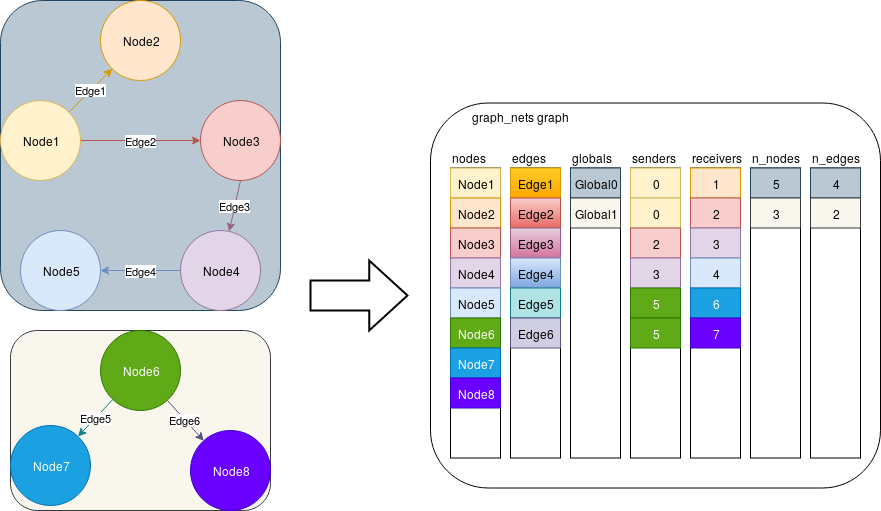
\includegraphics[width=150mm, keepaspectratio]{figures/transform_multiple.png}
	\caption{Graph transformation to GraphTuple format. The dictionary list is not visualized.}
	\label{fig:transform_multiple}
\end{figure}

On the Figure \ref{fig:transform_multiple} depicting this I also applied highlighting on the nodes, edges and graph backgrounds and the corresponding feature vectors and indices with the same color.

\FloatBarrier
%----------------------------------------------------------------------------
\section{Building the graphs}
%----------------------------------------------------------------------------

As I mentioned in the Introduction\ref{sect:Introduction} I used the stanfordnlp library to generate the universal dependency parse trees from the texts. Using the lemma and part of speech (POS) tag of the words I constructed the nodes of the graph the following way: if a word's lemma appears multiple times with the same POS tag in the text I've treated them as one node and the dependencies were merged as edges.

The feature vector a node is the vector of their lemma and POS tag. The feature vector of the edges is the UD relation between the words.

\begin{figure}[!ht]
	\centering
	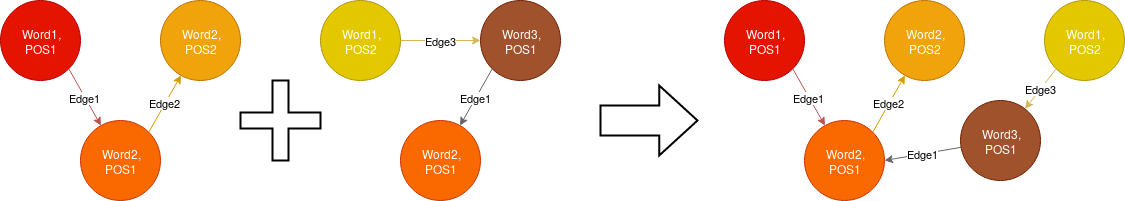
\includegraphics[width=150mm, keepaspectratio]{figures/merge_graphs_color.png}
	\caption{Graph merge.}
	\label{fig:merge_graph_color}
\end{figure}

As you can see at Figure \ref{fig:merge_graph_color}, the resulting graph is not a correct UD graph because the \textit{Word2, POS1} node has multiple incoming edges.

\begin{figure}[!ht]
	\centering
	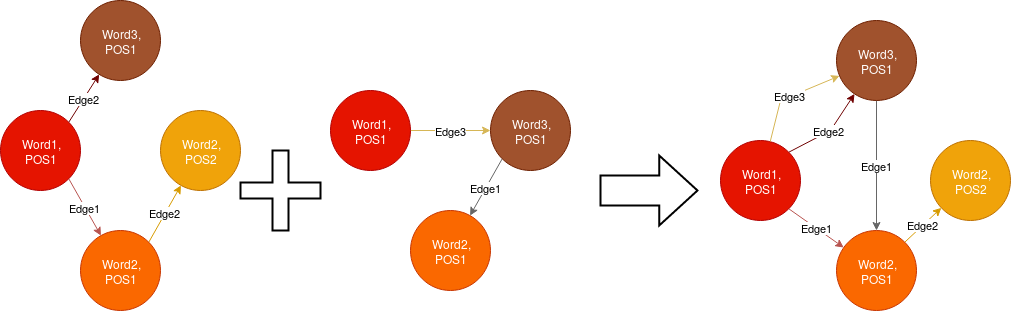
\includegraphics[width=150mm, keepaspectratio]{figures/merge_graphs_color_multiple.png}
	\caption{Graph merge with multiple matching nodes.}
	\label{fig:merge_graph_color_multiple}
\end{figure}

On Figure \ref{fig:merge_graph_color_multiple} you can see how multiple node matches affect the construction of the graph merging.

\begin{figure}[!ht]
	\centering
	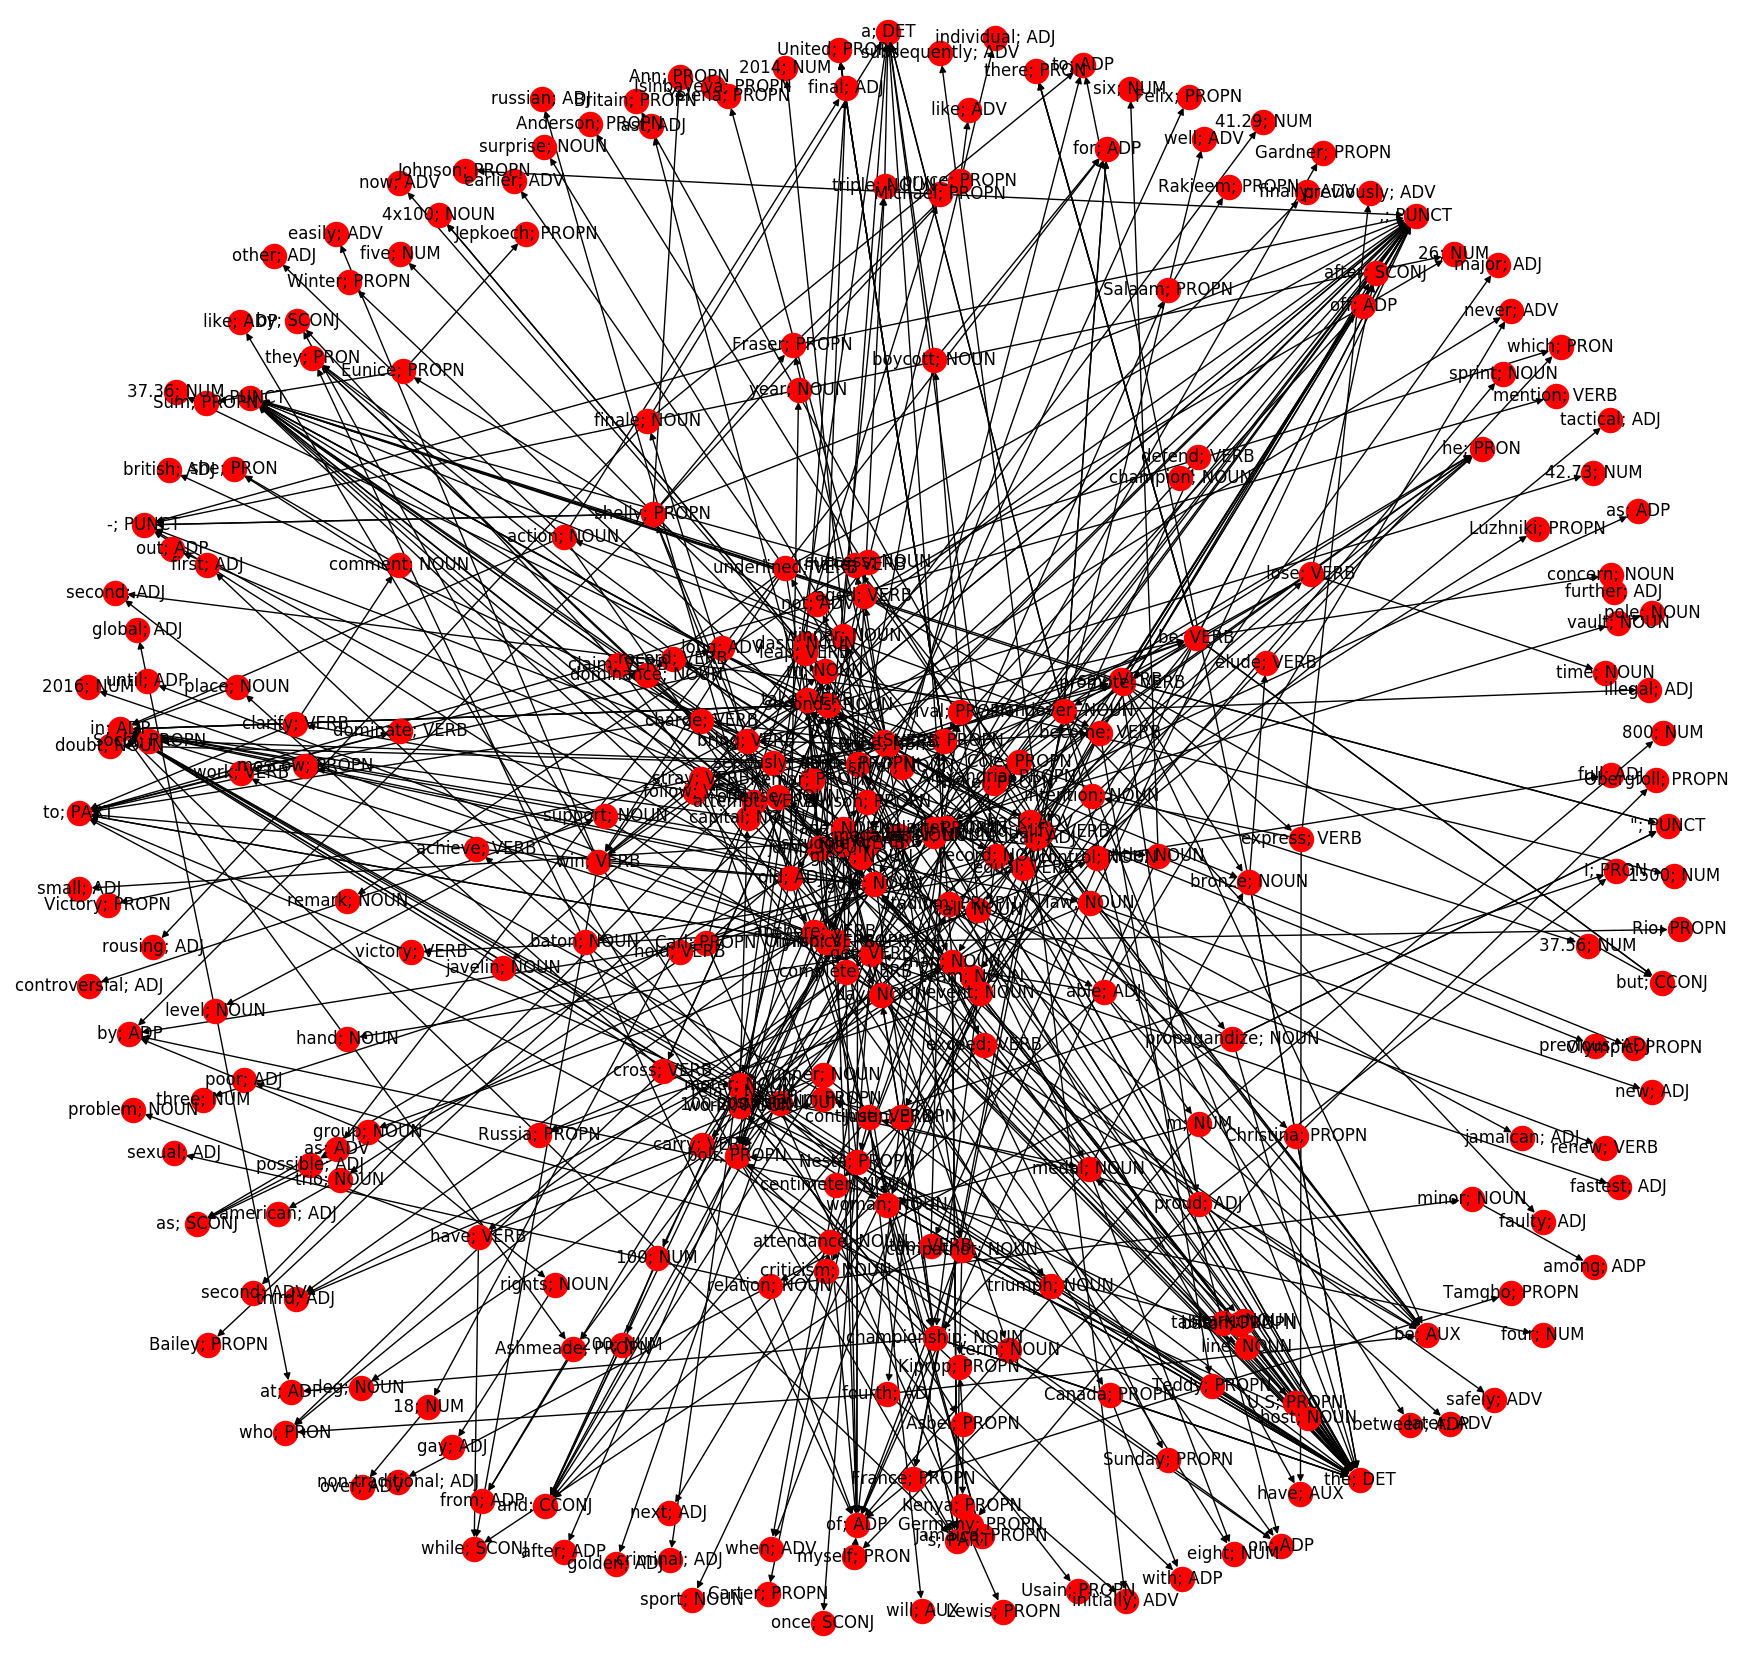
\includegraphics[width=150mm, keepaspectratio]{figures/usain_bolt_article.png}
	\caption{The graph built from the example article.}
	\label{fig:usain_article_graph}
\end{figure}

With this method I was able to represent an article with one large, merged graph, like the one on Figure \ref{fig:usain_article_graph}. As you can see, it is not easily interpretable for a human at first glance, but you can tell, that the nodes with high connectivity appeared frequently. Most of these are stop-words, which I left in the graphs for the connectivity.

\FloatBarrier
%----------------------------------------------------------------------------
\section{Forming the target graphs}
%----------------------------------------------------------------------------
Like I mentioned before, I needed the target graphs to be the same format as the input graph with the summary elements marked. Initially my approach was to try to learn the summaries written by people. For this I needed to generate summary graphs, but their structure was not adequate for training any graph neural network on it. So my solution was the following: I iterated through the edges of the article graph and if the sender node, the receiver node and the edge type matched any edge in the summary I've marked them by adding a 1.0 at the end of their feature vector. Otherwise I appended a 0.0 to the vector.

Similarly I iterated through the nodes as well and checked whether the same feature vector appears in the summary graph and appended 1.0 in case of successful search, 0.0 otherwise.

\begin{figure}[!ht]
	\centering
	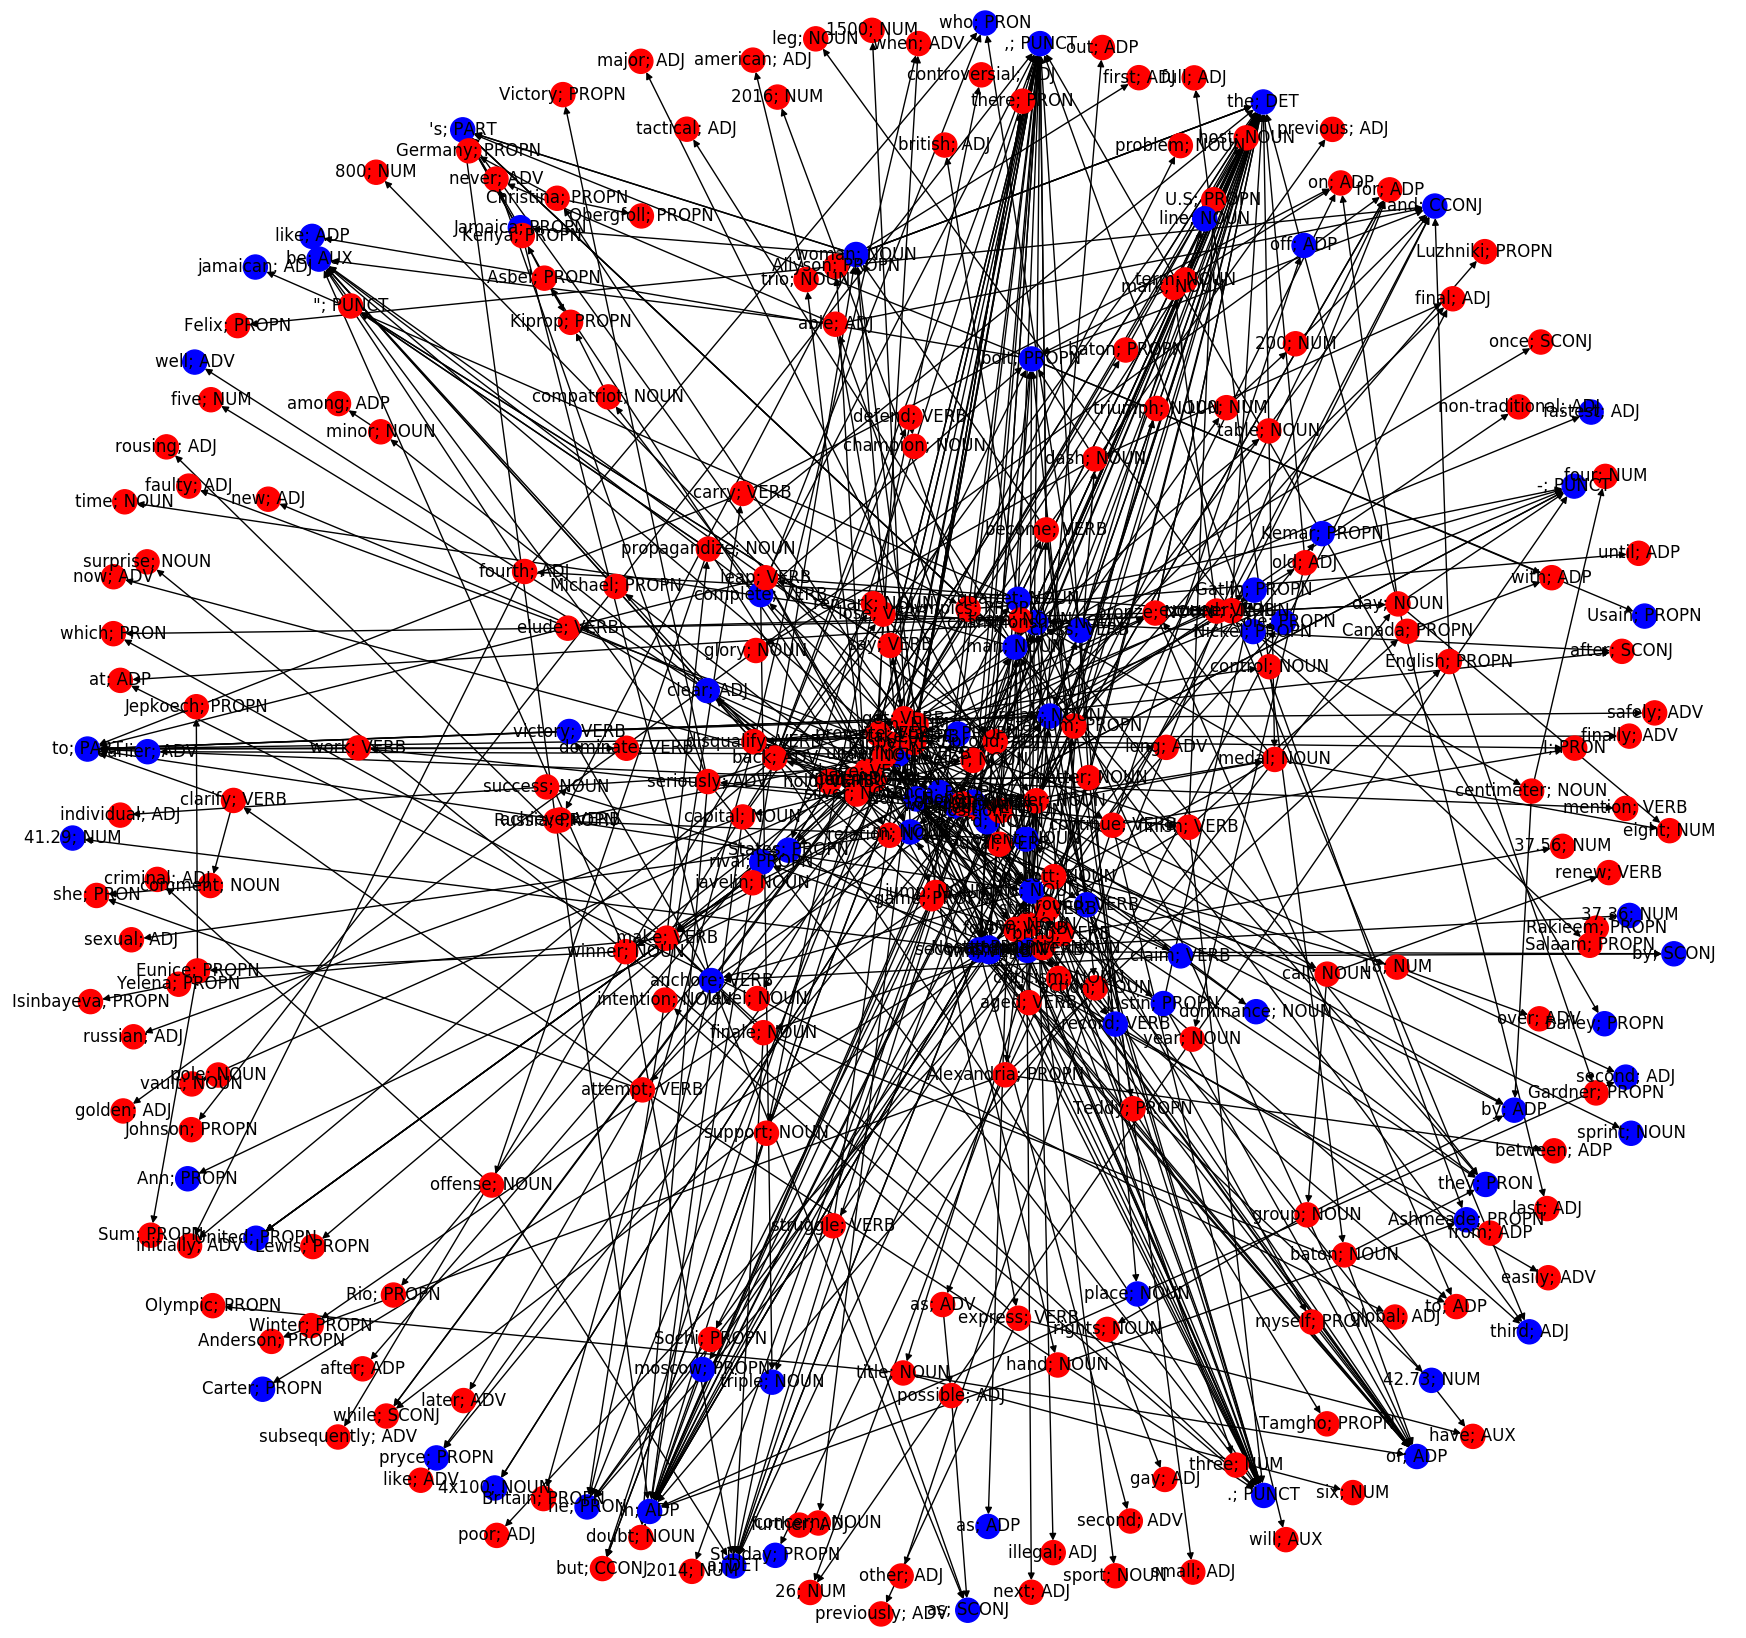
\includegraphics[width=150mm, keepaspectratio]{figures/usain_bolt_colored.png}
	\caption{The colored article graph of the example article. I highlighted the nodes with label 1 with blue.}
	\label{fig:usain_article_graph_colored}
\end{figure}

\begin{figure}[!ht]
	\centering
	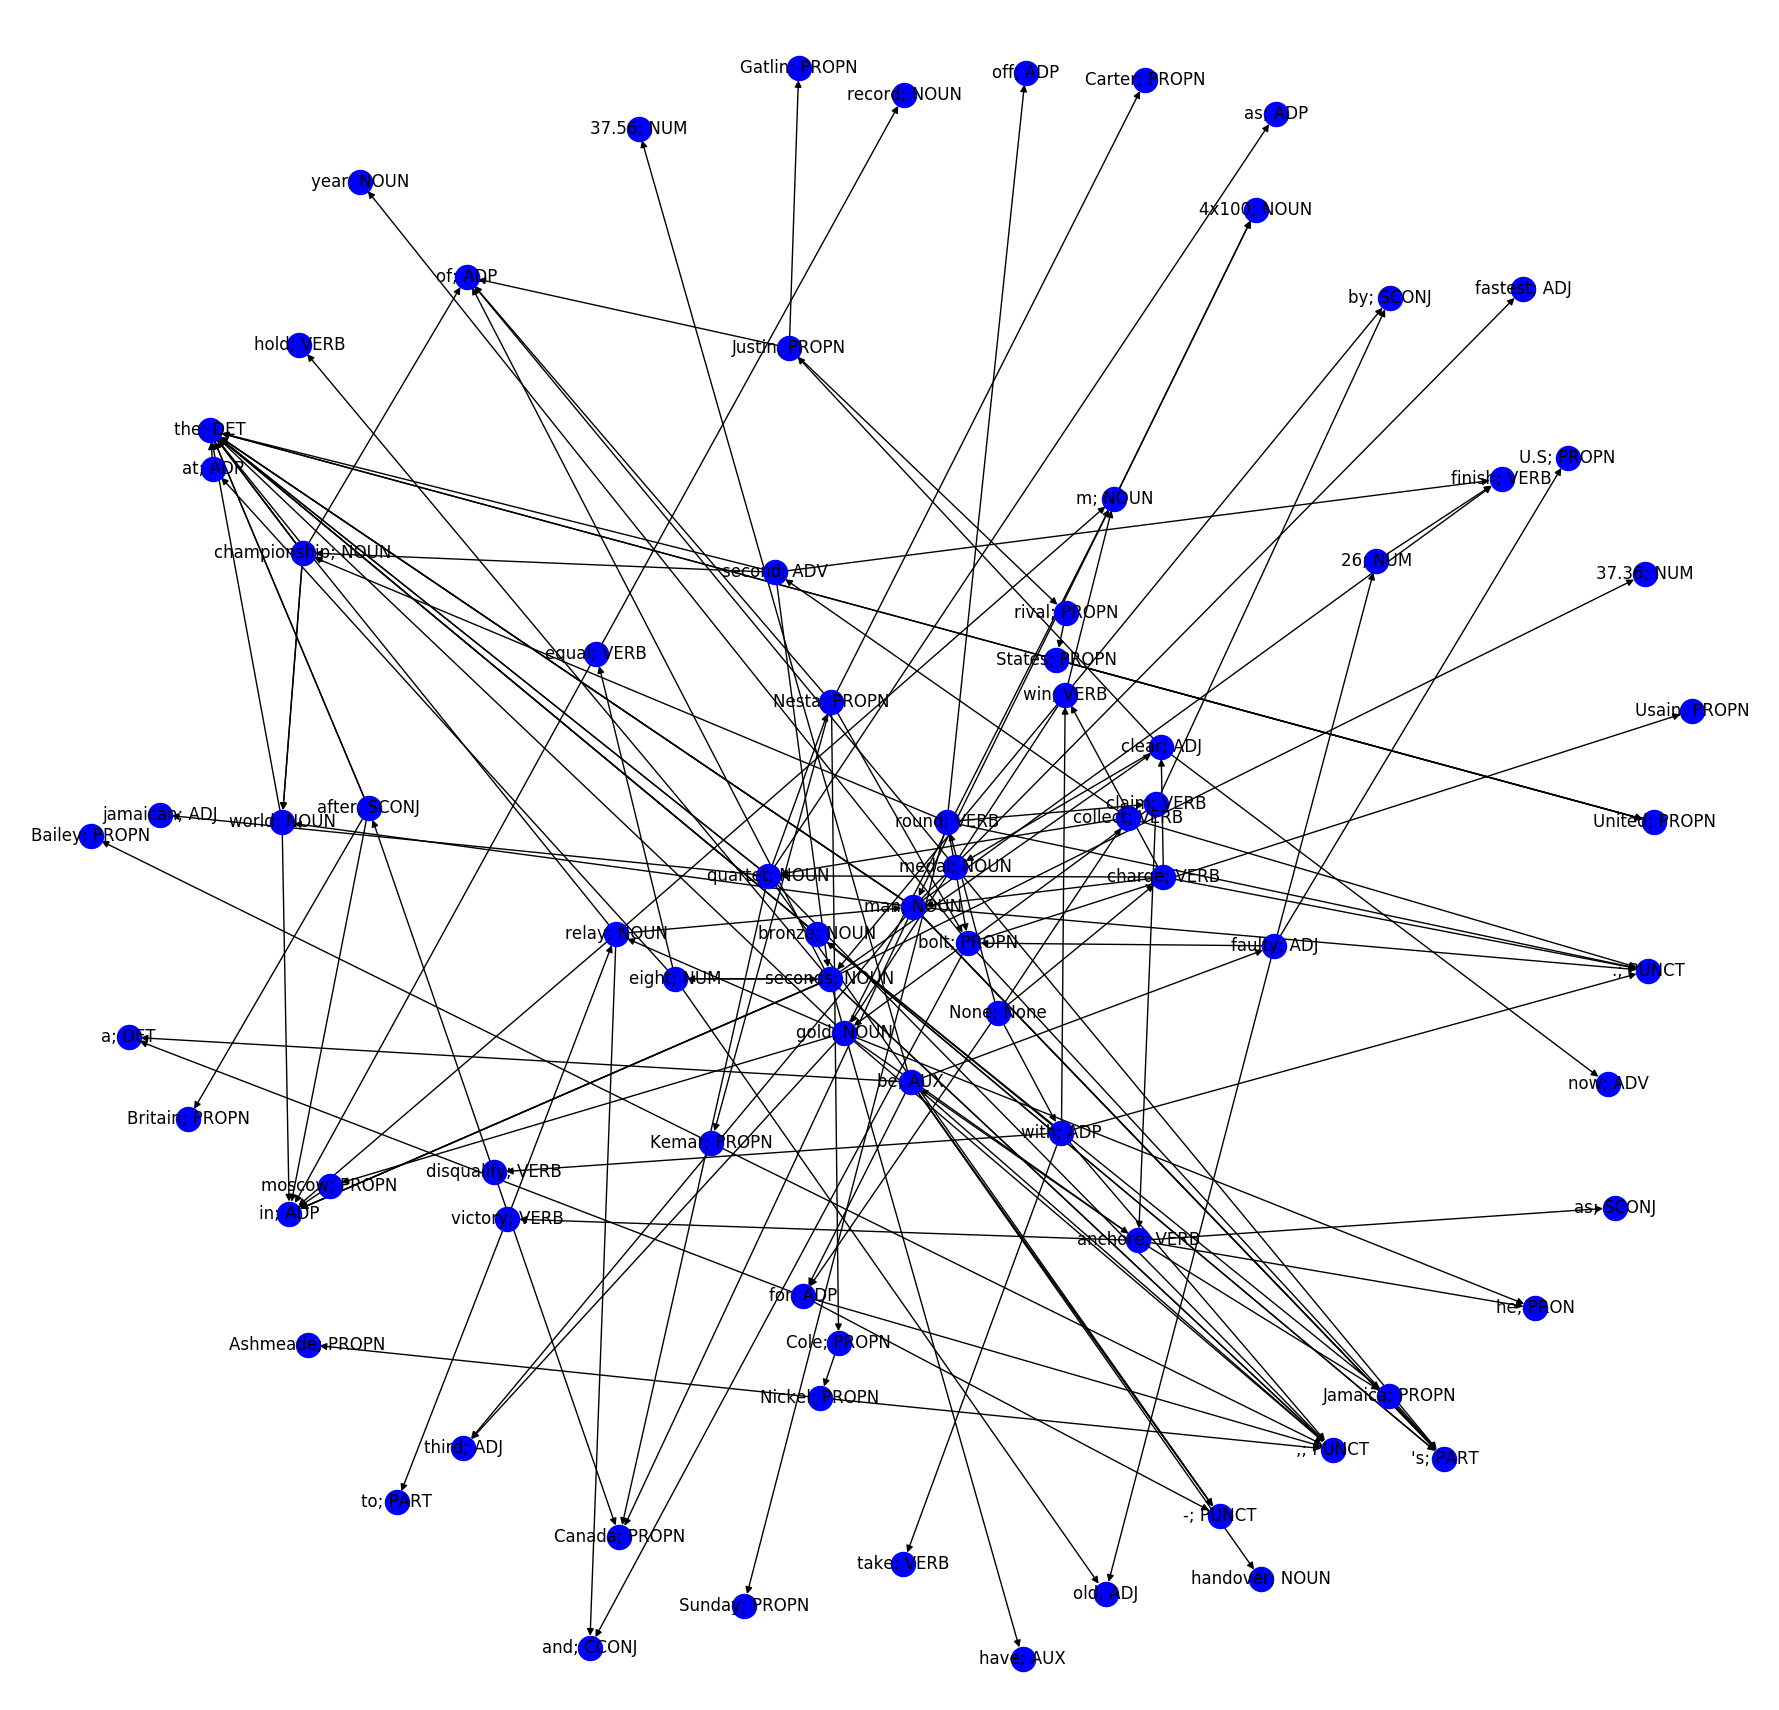
\includegraphics[width=150mm, keepaspectratio]{figures/usain_bolt_summary.png}
	\caption{The summary graph of the example article. This is the subgraph of the article graph with the node labels of 1.}
	\label{fig:usain_summary_graph}
\end{figure}

This way I was able to achieve the same structure, but with marked summary nodes and edges.

The problem with this approach was the fact, that some of the expressions used in the summary did not match up with anything from the original text so the result could not contain the same level of information as the summary graph on it's own.

However, the dataset contained the extracted summaries with the best possible ROUGE score and I decided to use that as the expected output of my neural network. The construction is similar to the previous one, but instead of generating another graph and then trying to find the corresponding parts I only iterated through the UD graphs of the sentences and labeled the nodes and edges in that with the right label.

The graphs resulting from this approach contained more information and proved to be better for training. On Figure \ref{fig:usain_article_graph_colored} and Figure \ref{fig:usain_summary_graph} you can see the results of the first article visualized in two different ways.
